\documentclass[sigconf]{acmart}

\usepackage{hyperref}

\usepackage{endfloat}
\renewcommand{\efloatseparator}{\mbox{}} % no new page between figures

\usepackage{booktabs} % For formal tables

\settopmatter{printacmref=false} % Removes citation information below abstract
\renewcommand\footnotetextcopyrightpermission[1]{} % removes footnote with conference information in first column
\pagestyle{plain} % removes running headers

\begin{document}
\title{Big Data Application in Web Search and Text Mining}


\author{Wenxuan Han}
% \orcid{1234-5678-9012}
\affiliation{%
  \institution{Indiana University Bloomingtonn}
  \streetaddress{1150 S Clarizz Blvd}
  \city{Bloomington} 
  \state{Indiana} 
  \postcode{47401-4294}
}
\email{wenxhan@iu.edu}

% The default list of authors is too long for headers}
% \renewcommand{\shortauthors}{B. Trovato et al.}


\begin{abstract}
Because of the rapid development of social media, there are gigantic amount of data generated in every second on the web. And those data could be stored in any forms like text, videos, images or their combinations. The more complicated forms of data, the more space it will take up and will cost more time to read it. Although most of today's personal computers have a very high performance, it is extremely difficult to process and analyze useful text information from those huge amount of unstructured data by using traditional single computer methods without the help of big data tools or text mining techniques. Fortunately, the improvements in big data application are also increasing fast in order to support those difficult works on web search and text mining. In this paper, we first study the data analytic steps in web search, then analyze some of the popular approaches or algorithms (e.g. Hubs, PageRank, etc), and at last, we discuss their applications in this field of big data.
\end{abstract}

\keywords{I523, HID209, Big Data, Social Media, Web Search, Text Mining, PageRank, Hubs}


\maketitle

\section{Introduction}

In recent years, social media has become more and more popular as a new way of communication and knowledge transfer. People could use it to create, share, exchange information and create their own network. Social media usage has been boosted from 2005 to 2015. Users between 18 and 29 ages are the mainly part of social media users \cite{editor01}. Today 90\% of young adults are active on social media. This proportion was 12\% in 2005 \cite{editor02}. And since the development of mobile products, social media has also been offered a better platform for users to share data faster and more convenient. Thus, this proportion could be keep stable or still increase during the next few years. \\ \\
Nowadays, a growing number of people prefer to express their opinion and feelings through tweeting, sharing images, commenting on social sites \cite{editor01}. Since the amount of such data become extremely large, it is significant to extract and analyze useful information through them by using text analysis methods. Therefore, some applications which based on these information have been developed, such as recommendation system and search engine. \\ \\
However, as the big data began to appear in the website, there are some problems we must face for web search which include the longer search queries (key words) requirement, support the huge number of searches and multiple languages. And these problems cause the progress of web search and text mining technologies. \\ \\
Web search is similar to information retrieval (IR) which is used to search for information on the World Wide Web \cite{editor05}. The information may be a mix of web pages, images, and other types of files. Since web search is applying on web, it has a much larger scale than many IR systems. Although web search is a complex technique, it has the capability to understand how to crawl internet to get and update information. \\ \\
Text mining (also known as knowledge discovery in text database \cite{editor04}) is semi-automatic process of discovering information, meaningful contents, topics, word, relations and patterns from a large amount of text data \cite{editor01}, which is also a branch of data mining. The text data could be extracted by web search at first.

\section{Web Search Technique}

\subsection{Key fundamental principles}
DIKW is the main part pf we. it the combination of Data, Information, Knowledge and Wisdom. For each element, it has the meaning.
Data: Raw web pages or "Dowuments views as a bag of words"
Information: Result of query or "Dowuments viewed as a collection of insight"


\begin{figure}
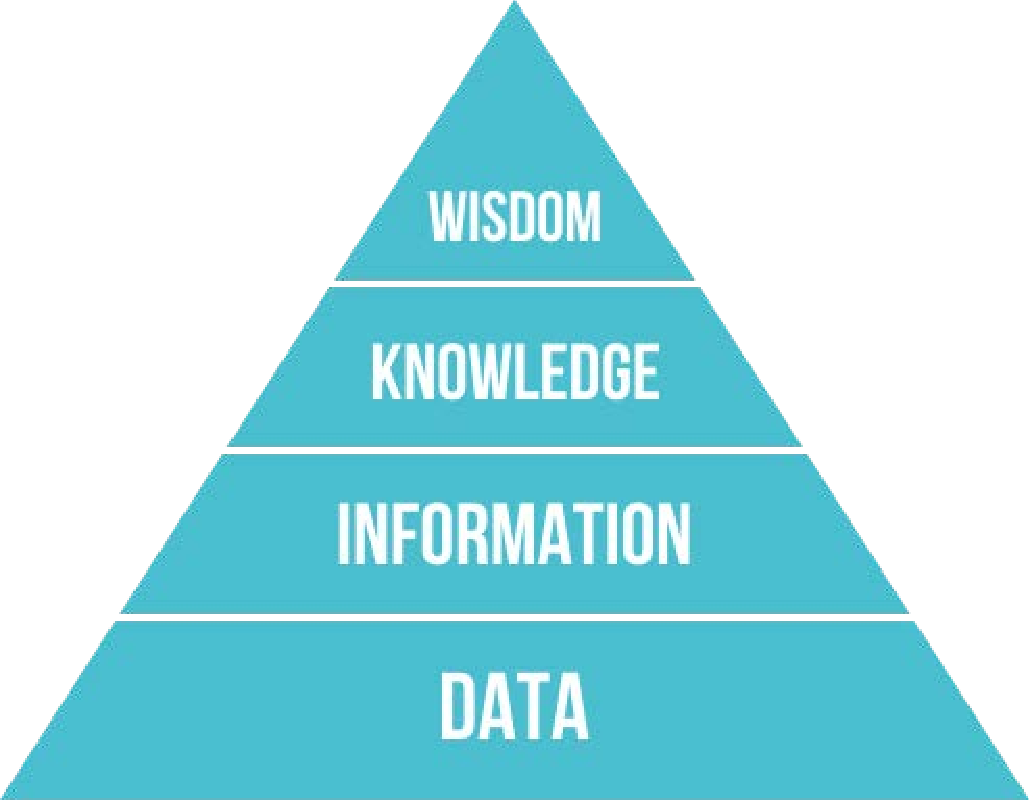
\includegraphics[width=0.30\columnwidth]{images/DIKW_Pyramid}
\caption{DIKW model.}
\end{figure}

\section{Text Mining}
\subsection{lala}
\begin{acks}

  The authors would like to thank 

\end{acks}

\bibliographystyle{ACM-Reference-Format}
\bibliography{report} 

\end{document}
